%Document-Author: Maino Elia
%Document-Date: 2016/05/29
%Document-Description: Documento di Definizione di prodotto del gruppo SWEeneyThreads 

\documentclass[a4paper]{article}
\usepackage[english, italian]{babel}
\usepackage[T1]{fontenc}
\usepackage[utf8]{inputenc}
\usepackage{url}
\usepackage{graphicx}
\usepackage[hidelinks]{hyperref}
\usepackage{booktabs}
\usepackage{eurosym}
\usepackage{tabularx}
\usepackage{pifont}
\usepackage[table]{xcolor}
\usepackage{float}
\usepackage[]{appendix}
\usepackage{ltxtable} 
\usepackage{geometry}
\geometry{margin=1in}
\usepackage{longtable}
\usepackage{multirow}

\graphicspath{{Immagini/DP/}}

\newcolumntype{Y}{>{\centering\arraybackslash}X}
\newcolumntype{s}{>{\hsize=.21\hsize}X}
\newcolumntype{f}{>{\hsize=.37\hsize}X}
\newcolumntype{m}{>{\hsize=.42\hsize}X}
\newcolumntype{t}{>{\hsize=.1\hsize}X}
\newcolumntype{r}{>{\hsize=.3\hsize}X}
\newcolumntype{k}{>{\hsize=.4\hsize}X}

\renewcommand{\abstractname}{Tabella contenuti}

\begin{document}
	
	\begin{titlepage}
		% Defines a new command for the horizontal lines, change thickness here
		\newcommand{\HRule}{\rule{\linewidth}{0.5mm}} 
		\center  
		
		% HEADING SECTION
		\textsc{\LARGE SWEeneyThreads}\\[1.5cm] 
		\textsc{\Large Actorbase}\\[0.5cm] 
		\textsc{\large a NoSQL DB based on the Actor model}\\[0.5cm]
		
		
		% TITLE SECTION
		\HRule \\[0.4cm]
		{ \huge \bfseries Definizione di prodotto}\\[0.4cm] 
		\HRule \\[1.5cm]
		
		% AUTHOR SECTION
		\begin{minipage}{0.4\textwidth}
			\begin{flushleft} \large
				\emph{Redattori:}\\
				Maino Elia \\
			\end{flushleft}
		\end{minipage}
		~
		\begin{minipage}{0.4\textwidth}
			\begin{flushright} \large
				\emph{Approvazione:} \\
                    \dots \\
				\emph{Verifica:} \\
                    \dots \\
				 
			\end{flushright}
		\end{minipage}
		
		%immagine
		\begin{figure}[H]
			\centering
			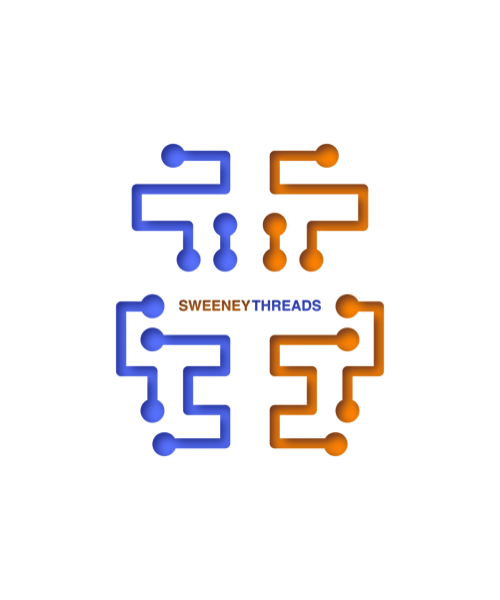
\includegraphics[scale=0.8]{sweeney.png}
		\end{figure}
		\begin{center}
			Versione 0.0.2
		\end{center}
		% Date, change the ->day to a set date if you want to be precise
		{\large \today} \\ [3cm] 
		% Fill the rest of the page with whitespace
		\vfill  
	\end{titlepage}
	
	
	\tableofcontents
	
	\newpage 
	\section*{Diario delle modifiche}
		\LTXtable{\textwidth}{Tabelle/tabelle_diario_modifiche/tabella_definizione.tex}

	\newpage \section{Introduzione}
	\subsection{Scopo del documento}
		Il documento illustra la progettazione di dettaglio del software \emph{Actorbase}.
		Le decisioni architetturali definite nel documento di \emph{Specifica Tecnica} saranno sviluppate ad un livello di dettaglio superiore, tale da fornire uno strumento adeguato a guidare e supportare l'attività di programmazione del gruppo.
	\subsection{Scopo del prodotto}
		Il progetto consiste nella realizzazione di un Database NoSQL key-value basato sul modello ad 
		Attori con l'obiettivo di fornire una tecnologia adatta allo sviluppo di moderne 
		applicazioni che richiedono brevissimi tempi di risposta e che elaborano enormi quantità 
		di dati. Lo sviluppo porterà al rilascio del software sotto licenza MIT.
	\subsection{Glossario}
		Al fine di evitare ambiguità di linguaggio e di massimizzare la comprensione dei documenti, il 
      gruppo ha steso un documento interno che è il \emph{Glossario v2.0.0}. In esso saranno definiti, in modo
      chiaro e conciso i termini che possono causare ambiguità o incomprensione del testo.
	\subsection{Riferimenti}
		\begin{itemize}
			\item \textbf{Slide dell'insegnamento Ingegneria del software mod.A:} \\
			\url{http://www.math.unipd.it/~tullio/IS-1/2015/Dispense/E02.pdf}
			\item \textbf{Scala:} \\
			\url{http://www.scala-lang.org/}
			\item \textbf{Java:} \\
			\url{http://www.java.com/}
			\item \textbf{Akka:} \\
			\url{http://akka.io/}
			\item \textbf{IntelliJ:} \\
			\url{http://www.jetbrains.com/idea/}
		\end{itemize}
	\textbf{Normativi}
		\begin{itemize}
			\item \textbf{Norme di progetto:} \emph{Norme di progetto v2.0.0}
			\item \textbf{Capitolato d'appalto Actorbase (C1):} \\ 
			\url{http://www.math.unipd.it/~tullio/IS-1/2015/Progetto/C1p.pdf}
		\end{itemize}
		
	\newpage	
	
	\section{Standard di progetto}
		Di seguito si riportano gli standard di progettazione e documentazione a cui i membri del gruppo dovranno attenersi durante l'attività di progettazione di dettaglio e programmazione.
	\subsection{Standard di progettazione}
		Gli standard di progettazione architetturale sono definiti nei documenti di \emph{Specifica Tecnica 3.0.0} e \emph{Norme di Progetto 3.0.0, sez 2.2.6}.  
	\subsection{Standard di codifica}
		Gli standard di codifica sono definiti nel documento \emph{Norme di Progetto 3.0.0, sez 2.2.11}.
	\subsection{Standard di documentazione del codice}
		Gli standard relativi alla documentazione del codice prodotto sono definiti nel documento \emph{Norme di progetto 3.0.0, sez 2.2.11}.
	\subsection{Strumenti di lavoro}
		Gli strumenti di lavoro da utilizzare sono definiti nel documento \emph{Norme di Progetto 3.0.0}.
		
	\newpage
	
	\section{Specifica componenti}
		In tale sezione verranno descritti il più dettagliatamente possibile i componenti architetturali definiti nel documento \emph{Specifica Tecnica}.
		
	\subsection{Actorbase}
		\begin{figure}[H]
			\centering
			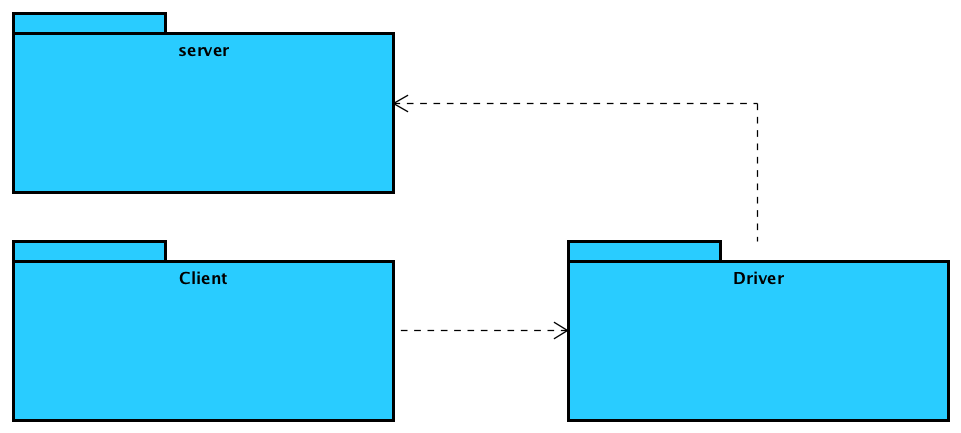
\includegraphics[width=\textwidth]{generalLevel.png}
			\caption{Actorbase architettura generale}
		\end{figure}
		L'architettura generale di \emph{Actorbase} è formata da tre componenti: Server, Client e Driver. 
		Il Client utilizza metodi e oggetti forniti dal Driver per comunicare con il Server.
		
	\subsection{Actorbase.server}
		\begin{figure}[H]
			\centering
			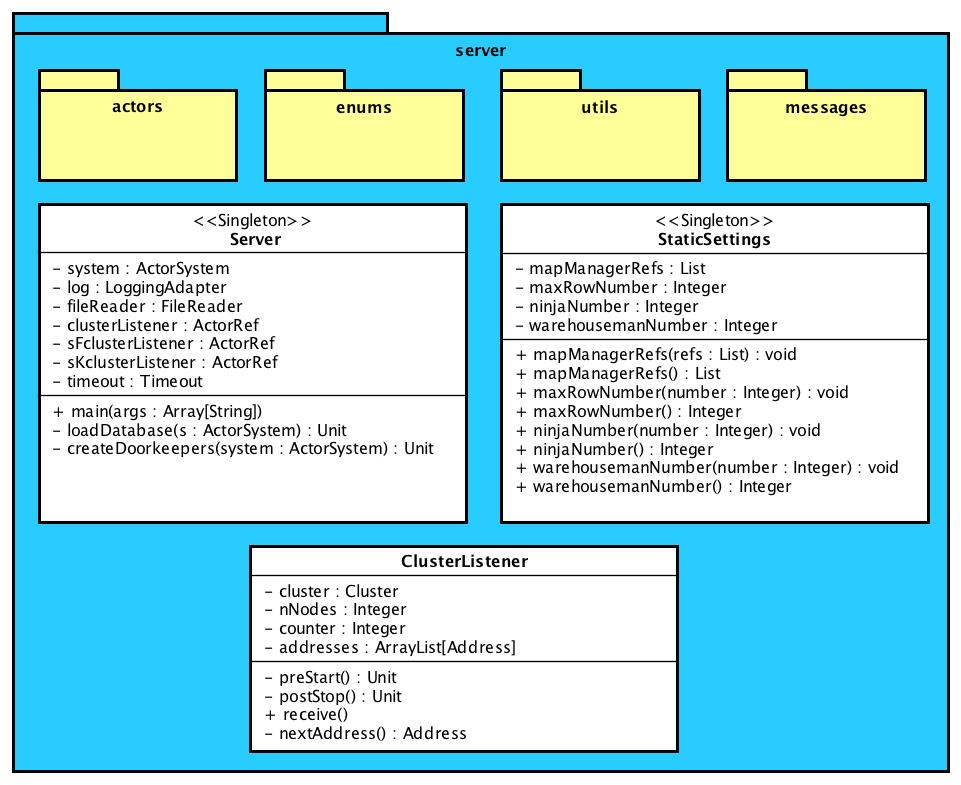
\includegraphics[scale=0.5]{Server/serverLevel.jpg}
			\caption{Componente Actorbase.server}
		\end{figure}
		La componente server di \emph{Actorbase} è il nucleo dell'applicativo, è composta dai packages: utils, messages, actors ed enums e dalla classe Server.
		
	\subsection{Actorbase.server.Server}
		\begin{figure}[H]
			\centering
			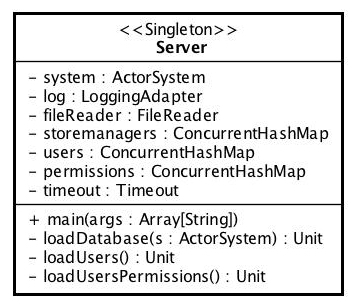
\includegraphics[scale=0.5]{Server/serverClass.jpg}
			\caption{Classe Actorbase.server.Server}
		\end{figure}
		\textbf{Descrizione}
			\\ \\
			Classe principale della parte Server del programma. \'E di fatto l'entry point dello stesso, gestisce la configurazione iniziale e avvia il sistema. Utilizza il design pattern Singleton.
			\\ \\
		\textbf{Utilizzo}
			\\ \\
			Classe che fornisce un punto di accesso al programma, la sua esecuzione avvia il server sulla macchina in cui viene lanciata.
			\\ \\
		\textbf{Classi ereditate}
			\\ \\
			Nessuna.
			\\ \\
		\textbf{Ereditata da}
			\\ \\
			Nessuna.
			\\ \\
		\textbf{Attributi}
			\begin{itemize}
				\item \texttt{system: ActorSystem } - Istanza di ActorSystem di Akka.
				\item \texttt{log: LoggingAdapter } - Permette di ottenere un log per l'ActorSystem.
				\item \texttt{fileReader: FileReader } - Accesso alla lettura di file.
				\item \texttt{storemanagers: ConcurrentHashMap[String, ActorRef] } - Mappa contenente la lista di attori di tipo UserManager presenti nel sistema.
				\item \texttt{users: ConcurrentHashMap[String, String] } - Mappa contenente la lista di utenti del sistema, le chiavi sono gli username degli utenti, i valori sono le password.
				\item \texttt{permissions: ConcurrentHashMap[String, UserPermission] } - Mappa che contiene per ogni utente la lista dei database a cui ha accesso.
				\item \texttt{timeout: Timeout } - Timeout di connessione.
			\end{itemize}
		\textbf{Metodi}
			\\ \\
			\texttt{main(args: Array[String]}
			\\ \\
			Metodo main che permette di avviare l'applicativo lato server. Si occupa di impostare i valori dei campi dati e di invocare gli altri metodi di configurazione presenti nella classe.
			\\ \\
			Lista parametri del metodo:
			\begin{itemize}
				\item \texttt{args: Array[String] } - Parametro standard del metodo main di \emph{Scala}.
			\end{itemize}
			\texttt{loadDatabases(s: ActorSystem): Unit}
			\\ \\
			Il metodo permette di caricare la lista dei database in memoria, inserendoli nella mappa \emph{storemanagers}. Non ritorna alcun valore.
			\\ \\
			Lista parametri del metodo:
			\begin{itemize}
				\item \texttt{s: ActorSystem } - ActorSystem da utilizzare per accedere agli attori necessari.
			\end{itemize}
			\texttt{loadUsers(): Unit}
			\\ \\
			Il metodo permette di caricare la lista di utenti in memoria, inserendoli nella mappa \emph{users}. Non ritorna alcun valore.
			\\ \\
			Lista parametri del metodo:
			\\ \\
			Nessuno.
			\\ \\
			\texttt{loadUsersPermissions(): Unit}
			\\ \\
			Il metodo permette di caricare la lista di permessi degli utenti in memoria, inserendoli nella mappa \emph{permissions}. Non ritorna alcun valore.
			\\ \\
			Lista parametri del metodo:
			\\ \\
			Nessuno.
	\subsection{Actorbase.server.utils}
		\begin{figure}[H]
			\centering
			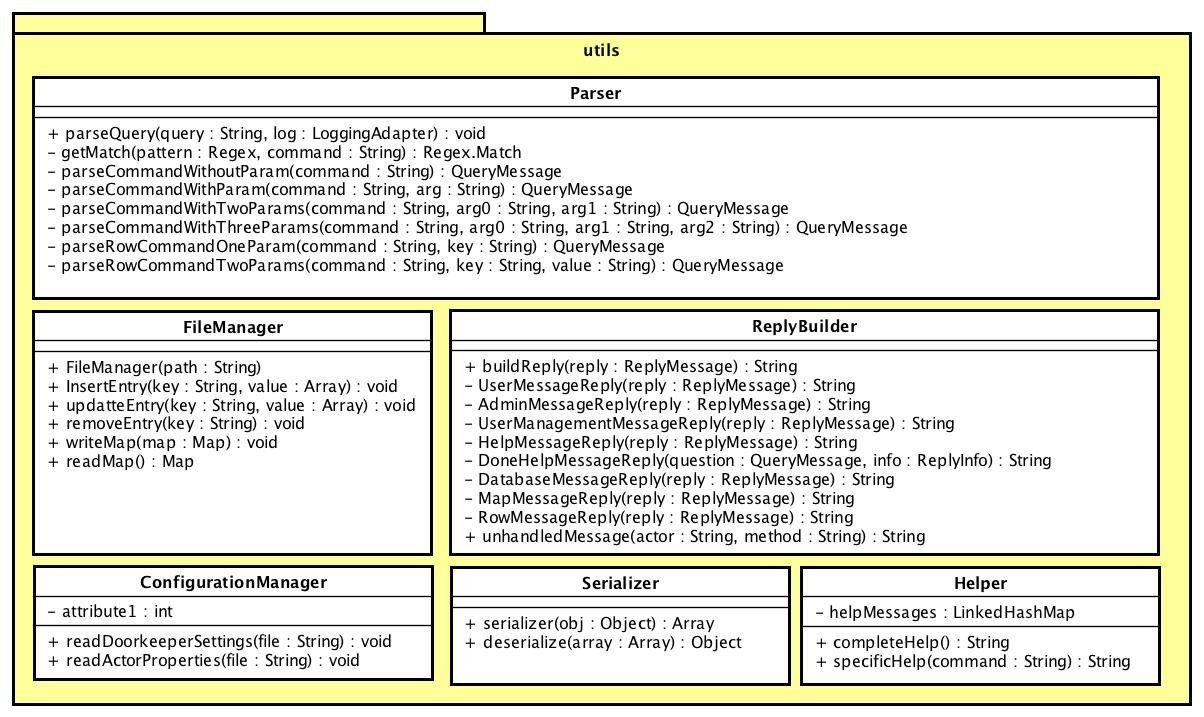
\includegraphics[width=\textwidth]{Server/utilsLevel.jpg}
			\caption{Componente Actorbase.server.utils}
		\end{figure}
		Package contenente le classi che effettuano operazioni varie a supporto delle varie componenti del server, e degli attori nello specifico.
		
			
	\subsection{Actorbase.server.utils.Parser}
		Immagine UML.
		\\ \\
		\textbf{Descrizione}
			\\ \\
			La classe \texttt{Parser} definisce i metodi per trasformare stringhe in messaggi \texttt{QueryMessage} utilizzabili dagli attori del sistema.
			\\ \\
		\textbf{Utilizzo}
			\\ \\
			Viene utilizzata da attori di tipo \texttt{Usermanager} per trasformare le richieste client in messaggi inviabili agli attori.
			\\ \\
		\textbf{Classi ereditate}
			\\ \\
			Nessuna.
			\\ \\
		\textbf{Ereditata da}
			\\ \\
			Nessuno.
			\\ \\
		\textbf{Attributi}
			\\ \\ 
			Nessuno.
			\\ \\
			\textbf{Costruttore: }\texttt{Parser()}
			\\ \\
			Costruttore senza parametri.
			\\ \\
			Lista parametri del metodo:
			\\ \\
			Nessuno.
			\\ \\
			\textbf{Metodo: }\texttt{parseQuery(query: String) : QueryMessage}
			\\ \\
			Effettua il parsing della stringa in base al numero di parametri che la compongono (utilizzando i metodi per il parsing a seconda dei parametri) e genera un \texttt{QueryMessage} che viene ritornato.
			\\ \\
			Lista parametri del metodo:
			\begin{itemize}
				\item \texttt{query: String } - Stringa da convertire in messaggio.
			\end{itemize}
			\textbf{Metodo: }\texttt{getMatch(pattern:Regex, command:String): Regex.Match}
			\\ \\
			Effettua il match dell'espressione regolare sulla stringa passata e ritorna il risultato.
			\\ \\
			Lista parametri del metodo:
			\begin{itemize}
				\item \texttt{pattern: Regex } - Pattern da utilizzare per il match.
				\item \texttt{command: String} - La stringa su cui effettuare il match.
			\end{itemize}
			\textbf{Metodo: }\texttt{parseCommandWithoutParam(command: String): QueryMessage}
			\\ \\
			Effettua il parsing di un comando senza parametri e ritorna il corrispondente \texttt{QueryMessage}.
			\\ \\
			Lista parametri del metodo:
			\begin{itemize}
				\item \texttt{command: String} - La stringa rappresentante il comando.
			\end{itemize}
			\textbf{Metodo: }\texttt{parseCommandWithParam(command: String, arg: String): QueryMessage}
			\\ \\
			Effettua il parsing di un comando con un parametro e ritorna il corrispondente \texttt{QueryMessage}.
			\\ \\
			Lista parametri del metodo:
			\begin{itemize}
				\item \texttt{command: String} - La stringa rappresentante il comando.
				\item \texttt{arg: String} - La stringa rappresentante il parametro.
			\end{itemize}
			\textbf{Metodo: }\texttt{parseCommandWithTwoParams(command:String, arg1: String, arg2: String):QueryMessage}
			\\ \\
			Effettua il parsing di un comando con due parametri e ritorna il corrispondente \texttt{QueryMessage}.
			\\ \\
			Lista parametri del metodo:
			\begin{itemize}
				\item \texttt{command: String} - La stringa rappresentante il comando.
				\item \texttt{arg1: String} - La stringa rappresentante il primo parametro.
				\item \texttt{arg2: String} - La stringa rappresentante il secondo parametro.
			\end{itemize}
			\textbf{Metodo: }\texttt{parseCommandWithThreeParams(command:String, arg1: String, arg2: String, arg3: String):QueryMessage}
			\\ \\
			Effettua il parsing di un comando con tre parametri e ritorna il corrispondente \texttt{QueryMessage}.
			\\ \\
			Lista parametri del metodo:
			\begin{itemize}
				\item \texttt{command: String} - La stringa rappresentante il comando.
				\item \texttt{arg1: String} - La stringa rappresentante il primo parametro.
				\item \texttt{arg2: String} - La stringa rappresentante il secondo parametro.
				\item \texttt{arg3: String} - La stringa rappresentante il terzo parametro.
			\end{itemize}
			\textbf{Metodo: }\texttt{parseRowCommandOneParam(command: String, key: String): QueryMessage}
			\\ \\
			Effettua il parsing di un comando al livello di item con un parametro (la chiave) e ritorna il corrispondente \texttt{QueryMessage}.
			\\ \\
			Lista parametri del metodo:
			\begin{itemize}
				\item \texttt{command: String} - La stringa rappresentante il comando a livello di item.
				\item \texttt{key: String} - La stringa rappresentante la chiave.
			\end{itemize}
			\textbf{Metodo: }\texttt{parseRowCommandTwoParams(command: String, key: String, value: String): QueryMessage}
			\\ \\
			Effettua il parsing di un comando al livello di item con due parametri (la chiave e il valore) e ritorna il corrispondente \texttt{QueryMessage}.
			\\ \\
			Lista parametri del metodo:
			\begin{itemize}
				\item \texttt{command: String} - La stringa rappresentante il comando a livello di item.
				\item \texttt{key: String} - La stringa rappresentante la chiave.
				\item \texttt{value: String} - La stringa rappresentante il valore.
			\end{itemize}
			
	\subsection{Actorbase.server.utils.FileManager}
		Immagine UML.
		\\ \\
		\textbf{Descrizione}
			\\ \\
			Classe che definisce i metodi per leggere e scrivere dati su disco.
			\\ \\
		\textbf{Utilizzo}
			\\ \\
			Viene utilizzata da attori di tipo \texttt{Warehouseman} per gestire la persistenza dei dati.
			\\ \\
		\textbf{Classi ereditate}
			\\ \\
			Nessuna.
			\\ \\
		\textbf{Ereditata da}
			\\ \\
			Nessuno.
			\\ \\
		\textbf{Attributi}
			\begin{itemize}
				\item \texttt{path: String } - Il percorso su cui effettuare le letture e le scritture.
				\item \dots
			\end{itemize}
		\textbf{Metodi}
			\\ \\
			\texttt{Firma del metodo}
			\\ \\
			Descrizione del metodo.
			\\ \\
			Lista parametri del metodo:
			\begin{itemize}
				\item \texttt{Nome parametro: tipo parametro } - Descrizione parametro
			\end{itemize}
			
	\subsection{Actorbase.server.utils.Helper}
		Immagine UML.
		\\ \\
		\textbf{Descrizione}
			\\ \\
			Classe che fornisce i metodi per ottenere una descrizione dei comandi di \emph{Actorbase}.
			\\ \\
		\textbf{Utilizzo}
			\\ \\
			Viene utilizzata per soddisfare una richiesta di \texttt{help} da parte di un utente.
			\\ \\
		\textbf{Classi ereditate}
			\\ \\
			Nessuna.
			\\ \\
		\textbf{Ereditata da}
			\\ \\
			Nessuno.
			\\ \\
		\textbf{Attributi}
			\begin{itemize}
				\item \texttt{helpMessages: LinkedHashMap[String, String] } - Mappa contenente i comandi come chiavi e le descrizioni degli stessi come valori.
			\end{itemize}
		\textbf{Metodo: }\texttt{completeHelp(): String}
			\\ \\
			Il metodo costruisce una stringa contenente l'aiuto completo, basandosi sugli elementi della mappa \texttt{helpMessages}.
			\\ \\
			Lista parametri del metodo:
			\\ \\
			Nessuno.
			\\ \\
		\textbf{Metodo: }\texttt{specificHelp(command: String): String}
			\\ \\
			Il metodo costruisce una stringa contenente l'aiuto per un comando specifico, basandosi sugli elementi della mappa \texttt{helpMessages}.
			\\ \\
			Lista parametri del metodo:
			\begin{itemize}
				\item \texttt{command: String } - Stringa rappresentante il comando per cui si vuole generare il messaggio di aiuto.
			\end{itemize}
			
	\subsection{Actorbase.server.utils.ConfigurationManager}
		Immagine UML.
		\\ \\
		\textbf{Descrizione}
			\\ \\
			Classe che fornisce i metodi di lettura e scrittura dei file di configurazione del server.
			\\ \\
		\textbf{Utilizzo}
			\\ \\
			Viene utilizzata per leggere le impostazioni del server dai file di configurazione all'avvio di esso. Inoltre viene utilizzata per scrivere modifiche alle configurazioni.
			\\ \\
		\textbf{Classi ereditate}
			\\ \\
			Nessuna.
			\\ \\
		\textbf{Ereditata da}
			\\ \\
			Nessuno.
			\\ \\
		\textbf{Attributi}
			\\ \\
			Nessuno.
			\\ \\
		\textbf{Metodo: }\texttt{readDoorkeepersSettings(fileName: String): util.HashMap[String, Integer]}
			\\ \\
			Il metodo legge dal file di configurazione gli indirizzi e le porte che attori di tipo \texttt{Doorkeeper} dovranno utilizzare per gestire le connessioni. Tali informazioni vengono ritornate con una mappa in cui le chiavi sono gli indirizzi e i valori sono le porte.
			\\ \\
			Lista parametri del metodo:
			\begin{itemize}
				\item \texttt{fileName: String} - Nome del file che contiene la configurazione dei \texttt{Doorkeeper}.
			\end{itemize}
		\textbf{Metodo: }\texttt{readActorsProperties(fileName: String): util.HashMap[ActorProperties, Integer]}
			\\ \\
			Il metodo legge dal file di configurazione le proprietà relative agli attori (come ad esempio il numero massimo di attori di tipo \texttt{Ninja}). Tali informazioni vengono ritornate con una mappa in cui le chiavi sono i nomi delle proprietà e i valori sono i valori di tali proprietà.
			\\ \\
			Lista parametri del metodo:
			\begin{itemize}
				\item \texttt{fileName: String} - Nome del file che contiene la configurazione degli attori.
			\end{itemize}
			
	\subsection{Actorbase.server.utils.ReplyBuilder}
		Immagine UML.
		\\ \\
		\textbf{Descrizione}
			\\ \\
			Classe che fornisce i metodi di creazione delle stringhe da mandare in risposta a richieste client.
			\\ \\
		\textbf{Utilizzo}
			\\ \\
			Viene utilizzata per costruire delle risposte in formato stringa a partire da messaggi. Tali risposte possono così essere inviate ad un client.
			\\ \\
		\textbf{Classi ereditate}
			\\ \\
			Nessuna.
			\\ \\
		\textbf{Ereditata da}
			\\ \\
			Nessuno.
			\\ \\
		\textbf{Attributi}
			\\ \\
			Nessuno.
			\\ \\
		\textbf{Metodo: }\texttt{buildReply(reply: ReplyMessage): String}
			\\ \\
			Il metodo permette di costruire una stringa a partire da un \texttt{ReplyMessage}. In particolare questo metodo si occupa di stabilire se il messaggio è di tipo amministratore o utente e delegare di conseguenza l'elaborazione al metodo più appropriato.
			Gestisce i seguenti messaggi:
			\begin{itemize}
				\item \texttt{UserMessage}
				\item \texttt{AdminMessage}
			\end{itemize}
			Lista parametri del metodo:
			\begin{itemize}
				\item \texttt{reply: ReplyMessage} - Il messaggio da cui ricavare la stringa.
			\end{itemize}
		\textbf{Metodo: }\texttt{UserMessageReply(reply: ReplyMessage): String}
			\\ \\
			Il metodo permette di costruire una stringa a partire da un \texttt{ReplyMessage}. In particolare questo metodo si occupa di stabilire che tipo di \texttt{UserMessage} si sia ricevuto.
			Gestisce i seguenti messaggi:
			\begin{itemize}
				\item \texttt{HelpMessage}
				\item \texttt{DatabaseMessage}
				\item \texttt{MapMessage}
				\item \texttt{RowMessage}
			\end{itemize}
			Lista parametri del metodo:
			\begin{itemize}
				\item \texttt{reply: ReplyMessage} - Il messaggio da cui ricavare la stringa.
			\end{itemize}
		\textbf{Metodo: }\texttt{AdminMessageReply(reply: ReplyMessage): String}
			\\ \\
			Il metodo permette di costruire una stringa a partire da un \texttt{ReplyMessage}. In particolare questo metodo si occupa di stabilire che tipo di \texttt{AdminMessage} si sia ricevuto.
			Gestisce i seguenti messaggi:
			\begin{itemize}
				\item \texttt{UsersManagementMessage}
				\item \texttt{PermissionsManagementMessage}
			\end{itemize}
			Lista parametri del metodo:
			\begin{itemize}
				\item \texttt{reply: ReplyMessage} - Il messaggio da cui ricavare la stringa.
			\end{itemize}
		\textbf{Metodo: }\texttt{UserManagementMessageReply(reply: ReplyMessage): String}
			\\ \\
			Il metodo permette di costruire una stringa a partire da un \texttt{ReplyMessage}. In particolare questo metodo si occupa di gestire messaggi di tipo \texttt{UsersManagementMessage}.
			Gestisce i seguenti messaggi:
			\begin{itemize}
				\item \texttt{ListUserMessage}
				\item \texttt{AddUserMessage}
				\item \texttt{RemoveUserMessage}
			\end{itemize}
			Lista parametri del metodo:
			\begin{itemize}
				\item \texttt{reply: ReplyMessage} - Il messaggio da cui ricavare la stringa.
			\end{itemize}
		\textbf{Metodo: }\texttt{PermissionsManagementMessageReply(reply: ReplyMessage): String}
			\\ \\
			Il metodo permette di costruire una stringa a partire da un \texttt{ReplyMessage}. In particolare questo metodo si occupa di gestire messaggi di tipo \texttt{PermissionManagementMessage}.
			Gestisce i seguenti messaggi:
			\begin{itemize}
				\item \texttt{ListPermissionMessage}
				\item \texttt{AddPermissionMessage}
				\item \texttt{RemovePermissionMessage}
			\end{itemize}
			Lista parametri del metodo:
			\begin{itemize}
				\item \texttt{reply: ReplyMessage} - Il messaggio da cui ricavare la stringa.
			\end{itemize}
		\textbf{Metodo: }\texttt{HelpMessageReply(reply: ReplyMessage): String}
			\\ \\
			Il metodo permette di costruire una stringa a partire da un \texttt{ReplyMessage}. In particolare questo metodo si occupa di gestire messaggi di tipo \texttt{HelpMessage} invocando gli opportuni metodi.
			Gestisce i seguenti messaggi:
			\begin{itemize}
				\item \texttt{HelpMessage}
			\end{itemize}
			Lista parametri del metodo:
			\begin{itemize}
				\item \texttt{reply: ReplyMessage} - Il messaggio da cui ricavare la stringa.
			\end{itemize}
		\textbf{Metodo: }\texttt{DoneHelpMessageReply(question: QueryMessage, info: ReplyInfo): String}
			\\ \\
			Il metodo permette di costruire una stringa a partire da un \texttt{ReplyMessage}. In particolare questo metodo si occupa di gestire messaggi di tipo \texttt{HelpMessage} maggiormente nel dettaglio.
			Gestisce i seguenti messaggi:
			\begin{itemize}
				\item \texttt{CompleteHelpMessage}
				\item \texttt{SpecificHelpMessage}
			\end{itemize}
			Lista parametri del metodo:
			\begin{itemize}
				\item \texttt{reply: ReplyMessage} - Il messaggio da cui ricavare la stringa.
			\end{itemize}
		\textbf{Metodo: }\texttt{DatabaseMessageReply(reply: ReplyMessage): String}
			\\ \\
			Il metodo permette di costruire una stringa a partire da un \texttt{ReplyMessage}. In particolare questo metodo si occupa di gestire messaggi di tipo \texttt{DatabaseMessage}.
			Gestisce i seguenti messaggi:
			\begin{itemize}
				\item \texttt{ListDatabaseMessage}
				\item \texttt{SelectDatabaseMessage}
				\item \texttt{CreateDatabaseMessage}
				\item \texttt{DeleteDatabaseMessage}
			\end{itemize}
			Lista parametri del metodo:
			\begin{itemize}
				\item \texttt{reply: ReplyMessage} - Il messaggio da cui ricavare la stringa.
			\end{itemize}
		\textbf{Metodo: }\texttt{MapMessageReply(reply: ReplyMessage): String}
			\\ \\
			Il metodo permette di costruire una stringa a partire da un \texttt{ReplyMessage}. In particolare questo metodo si occupa di gestire messaggi di tipo \texttt{MapMessage}.
			Gestisce i seguenti messaggi:
			\begin{itemize}
				\item \texttt{ListMapMessage}
				\item \texttt{SelectMapMessage}
				\item \texttt{CreateMapMessage}
				\item \texttt{DeleteMapMessage}
			\end{itemize}
			Lista parametri del metodo:
			\begin{itemize}
				\item \texttt{reply: ReplyMessage} - Il messaggio da cui ricavare la stringa.
			\end{itemize}
		\textbf{Metodo: }\texttt{RowMessageReply(reply: ReplyMessage): String}
			\\ \\
			Il metodo permette di costruire una stringa a partire da un \texttt{ReplyMessage}. In particolare questo metodo si occupa di gestire messaggi di tipo \texttt{RowMessage}.
			Gestisce i seguenti messaggi:
			\begin{itemize}
				\item \texttt{ListKeysMessage}
				\item \texttt{FindRowMessage}
				\item \texttt{InsertRowMessage}
				\item \texttt{UpdateRowMessage}
				\item \texttt{RemoveRowMessage}
			\end{itemize}
			Lista parametri del metodo:
			\begin{itemize}
				\item \texttt{reply: ReplyMessage} - Il messaggio da cui ricavare la stringa.
			\end{itemize}
		\textbf{Metodo: }\texttt{unhandledMessage(actor: String, method: String): String}
			\\ \\
			Il metodo permette di costruire una stringa per i messaggi che non sono stati gestiti.
			Lista parametri del metodo:
			\begin{itemize}
				\item \texttt{actor: String} - Il percorso dell'attore che non ha gestito il messaggio
				\item \texttt{method: String} - Il nome del metodo in cui non è stato gestito il messaggio
			\end{itemize}
			
	\subsection{Actorbase.server.utils.Serializer}
		Immagine UML.
		\\ \\
		\textbf{Descrizione}
			\\ \\
			Classe che gestisce la serializzazione e la deserializzazione di oggetti.
			\\ \\
		\textbf{Utilizzo}
			\\ \\
			Viene utilizzata per serializzare e deserializzare oggetti in Array di Byte in modo da poterli trattare come dati di \emph{Actorbase}.
			\\ \\
		\textbf{Classi ereditate}
			\\ \\
			Nessuna.
			\\ \\
		\textbf{Ereditata da}
			\\ \\
			Nessuno.
			\\ \\
		\textbf{Attributi}
			\\ \\
			Nessuno.
			\\ \\
		\textbf{Metodo: }\texttt{serialize(obj: Object): Array[Byte]}
			\\ \\
			Il metodo serializza un oggetto in un array di Byte.
			\\ \\
			Lista parametri del metodo:
			\begin{itemize}
				\item \texttt{obj: Object} - L'oggetto da serializzare.
			\end{itemize}
		\textbf{Metodo: }\texttt{deserialize(array: Array[Byte]): Object}
			\\ \\
			Il metodo genera un Oggetto a partire da un array di Byte.
			\\ \\
			Lista parametri del metodo:
			\begin{itemize}
				\item \texttt{array: Array[Byte]} - L'array da utilizzare per generare l'oggetto.
			\end{itemize}
			
	\subsection{Actorbase.server.actors}
		Immagine UML del package e breve descrizione.
		
	\subsection{Actorbase.server.actors.Doorkeeper}
		Immagine UML.
		\\ \\
		\textbf{Descrizione}
			\\ \\
			Descrizione testuale.
			\\ \\
		\textbf{Utilizzo}
			\\ \\
			Descrizione testuale.
			\\ \\
		\textbf{Classi ereditate}
			\begin{itemize}
				\item Classe
				\item \dots
			\end{itemize}
		\textbf{Ereditata da}
			\begin{itemize}
				\item Classe
				\item \dots
			\end{itemize}
		\textbf{Attributi}
			\begin{itemize}
				\item \texttt{Nome attributo: tipo attributo } - Descrizione attributo
				\item \dots
			\end{itemize}
		\textbf{Metodi}
			\\ \\
			\texttt{Firma del metodo}
			\\ \\
			Descrizione del metodo.
			\\ \\
			Lista parametri del metodo:
			\begin{itemize}
				\item \texttt{Nome parametro: tipo parametro } - Descrizione parametro
			\end{itemize}
			
	\subsection{Actorbase.server.actors.Usermanager}
		Immagine UML.
		\\ \\
		\textbf{Descrizione}
			\\ \\
			Descrizione testuale.
			\\ \\
		\textbf{Utilizzo}
			\\ \\
			Descrizione testuale.
			\\ \\
		\textbf{Classi ereditate}
			\begin{itemize}
				\item Classe
				\item \dots
			\end{itemize}
		\textbf{Ereditata da}
			\begin{itemize}
				\item Classe
				\item \dots
			\end{itemize}
		\textbf{Attributi}
			\begin{itemize}
				\item \texttt{Nome attributo: tipo attributo } - Descrizione attributo
				\item \dots
			\end{itemize}
		\textbf{Metodi}
			\\ \\
			\texttt{Firma del metodo}
			\\ \\
			Descrizione del metodo.
			\\ \\
			Lista parametri del metodo:
			\begin{itemize}
				\item \texttt{Nome parametro: tipo parametro } - Descrizione parametro
			\end{itemize}
			
	\subsection{Actorbase.server.actors.Main}
		Immagine UML.
		\\ \\
		\textbf{Descrizione}
			\\ \\
			Descrizione testuale.
			\\ \\
		\textbf{Utilizzo}
			\\ \\
			Descrizione testuale.
			\\ \\
		\textbf{Classi ereditate}
			\begin{itemize}
				\item Classe
				\item \dots
			\end{itemize}
		\textbf{Ereditata da}
			\begin{itemize}
				\item Classe
				\item \dots
			\end{itemize}
		\textbf{Attributi}
			\begin{itemize}
				\item \texttt{Nome attributo: tipo attributo } - Descrizione attributo
				\item \dots
			\end{itemize}
		\textbf{Metodi}
			\\ \\
			\texttt{Firma del metodo}
			\\ \\
			Descrizione del metodo.
			\\ \\
			Lista parametri del metodo:
			\begin{itemize}
				\item \texttt{Nome parametro: tipo parametro } - Descrizione parametro
			\end{itemize}
			
	\subsection{Actorbase.server.actors.Storemanager}
		Immagine UML.
		\\ \\
		\textbf{Descrizione}
			\\ \\
			Descrizione testuale.
			\\ \\
		\textbf{Utilizzo}
			\\ \\
			Descrizione testuale.
			\\ \\
		\textbf{Classi ereditate}
			\begin{itemize}
				\item Classe
				\item \dots
			\end{itemize}
		\textbf{Ereditata da}
			\begin{itemize}
				\item Classe
				\item \dots
			\end{itemize}
		\textbf{Attributi}
			\begin{itemize}
				\item \texttt{Nome attributo: tipo attributo } - Descrizione attributo
				\item \dots
			\end{itemize}
		\textbf{Metodi}
			\\ \\
			\texttt{Firma del metodo}
			\\ \\
			Descrizione del metodo.
			\\ \\
			Lista parametri del metodo:
			\begin{itemize}
				\item \texttt{Nome parametro: tipo parametro } - Descrizione parametro
			\end{itemize}
		
	\subsection{Actorbase.server.actors.Storefinder}
		Immagine UML.
		\\ \\
		\textbf{Descrizione}
			\\ \\
			Descrizione testuale.
			\\ \\
		\textbf{Utilizzo}
			\\ \\
			Descrizione testuale.
			\\ \\
		\textbf{Classi ereditate}
			\begin{itemize}
				\item Classe
				\item \dots
			\end{itemize}
		\textbf{Ereditata da}
			\begin{itemize}
				\item Classe
				\item \dots
			\end{itemize}
		\textbf{Attributi}
			\begin{itemize}
				\item \texttt{Nome attributo: tipo attributo } - Descrizione attributo
				\item \dots
			\end{itemize}
		\textbf{Metodi}
			\\ \\
			\texttt{Firma del metodo}
			\\ \\
			Descrizione del metodo.
			\\ \\
			Lista parametri del metodo:
			\begin{itemize}
				\item \texttt{Nome parametro: tipo parametro } - Descrizione parametro
			\end{itemize}
			
	\subsection{Actorbase.server.actors.Storekeeper}
		Immagine UML.
		\\ \\
		\textbf{Descrizione}
			\\ \\
			Descrizione testuale.
			\\ \\
		\textbf{Utilizzo}
			\\ \\
			Descrizione testuale.
			\\ \\
		\textbf{Classi ereditate}
			\begin{itemize}
				\item Classe
				\item \dots
			\end{itemize}
		\textbf{Ereditata da}
			\begin{itemize}
				\item Classe
				\item \dots
			\end{itemize}
		\textbf{Attributi}
			\begin{itemize}
				\item \texttt{Nome attributo: tipo attributo } - Descrizione attributo
				\item \dots
			\end{itemize}
		\textbf{Metodi}
			\\ \\
			\texttt{Firma del metodo}
			\\ \\
			Descrizione del metodo.
			\\ \\
			Lista parametri del metodo:
			\begin{itemize}
				\item \texttt{Nome parametro: tipo parametro } - Descrizione parametro
			\end{itemize}
			
	\subsection{Actorbase.server.actors.Warehouseman}
		Immagine UML.
		\\ \\
		\textbf{Descrizione}
			\\ \\
			Descrizione testuale.
			\\ \\
		\textbf{Utilizzo}
			\\ \\
			Descrizione testuale.
			\\ \\
		\textbf{Classi ereditate}
			\begin{itemize}
				\item Classe
				\item \dots
			\end{itemize}
		\textbf{Ereditata da}
			\begin{itemize}
				\item Classe
				\item \dots
			\end{itemize}
		\textbf{Attributi}
			\begin{itemize}
				\item \texttt{Nome attributo: tipo attributo } - Descrizione attributo
				\item \dots
			\end{itemize}
		\textbf{Metodi}
			\\ \\
			\texttt{Firma del metodo}
			\\ \\
			Descrizione del metodo.
			\\ \\
			Lista parametri del metodo:
			\begin{itemize}
				\item \texttt{Nome parametro: tipo parametro } - Descrizione parametro
			\end{itemize}
			
	\subsection{Actorbase.server.enums}
		Immagine UML del package e breve descrizione.
		
	\subsection{Actorbase.server.enums.Permission (trait)}
		Immagine UML.
		\\ \\
		\textbf{Descrizione}
			\\ \\
			Descrizione testuale.
			\\ \\
		\textbf{Utilizzo}
			\\ \\
			Descrizione testuale.
			\\ \\
		\textbf{Classi ereditate}
			\begin{itemize}
				\item Classe
				\item \dots
			\end{itemize}
		\textbf{Ereditata da}
			\begin{itemize}
				\item Classe
				\item \dots
			\end{itemize}
		\textbf{Attributi}
			\begin{itemize}
				\item \texttt{Nome attributo: tipo attributo } - Descrizione attributo
				\item \dots
			\end{itemize}
		\textbf{Metodi}
			\\ \\
			Nessuno.
		
	\subsection{Actorbase.server.enums.ReplyResult (trait)}
		Immagine UML.
		\\ \\
		\textbf{Descrizione}
			\\ \\
			Descrizione testuale.
			\\ \\
		\textbf{Utilizzo}
			\\ \\
			Descrizione testuale.
			\\ \\
		\textbf{Classi ereditate}
			\begin{itemize}
				\item Classe
				\item \dots
			\end{itemize}
		\textbf{Ereditata da}
			\begin{itemize}
				\item Classe
				\item \dots
			\end{itemize}
		\textbf{Attributi}
			\begin{itemize}
				\item \texttt{Nome attributo: tipo attributo } - Descrizione attributo
				\item \dots
			\end{itemize}
		\textbf{Metodi}
			\\ \\
			Nessuno.
			
	\subsection{Actorbase.server.enums.Read}
		Immagine UML.
		\\ \\
		\textbf{Descrizione}
			\\ \\
			Descrizione testuale.
			\\ \\
		\textbf{Utilizzo}
			\\ \\
			Descrizione testuale.
			\\ \\
		\textbf{Classi ereditate}
			\begin{itemize}
				\item Classe
				\item \dots
			\end{itemize}
		\textbf{Ereditata da}
			\begin{itemize}
				\item Classe
				\item \dots
			\end{itemize}
		\textbf{Attributi}
			\begin{itemize}
				\item \texttt{Nome attributo: tipo attributo } - Descrizione attributo
				\item \dots
			\end{itemize}
		\textbf{Metodi}
			\\ \\
			Nessuno.
			
	\subsection{Actorbase.server.enums.Write}
		Immagine UML.
		\\ \\
		\textbf{Descrizione}
			\\ \\
			Descrizione testuale.
			\\ \\
		\textbf{Utilizzo}
			\\ \\
			Descrizione testuale.
			\\ \\
		\textbf{Classi ereditate}
			\begin{itemize}
				\item Classe
				\item \dots
			\end{itemize}
		\textbf{Ereditata da}
			\begin{itemize}
				\item Classe
				\item \dots
			\end{itemize}
		\textbf{Attributi}
			\begin{itemize}
				\item \texttt{Nome attributo: tipo attributo } - Descrizione attributo
				\item \dots
			\end{itemize}
		\textbf{Metodi}
			\\ \\
			Nessuno.
	
		Immagine UML.
		\textbf{Descrizione}
			Descrizione testuale.
		\textbf{Utilizzo}
			Descrizione testuale.
		\textbf{Classi ereditate}
			\begin{itemize}
				\item Classe
				\item \dots
			\end{itemize}
		\textbf{Ereditata da}
			\begin{itemize}
				\item Classe
				\item \dots
			\end{itemize}
		\textbf{Attributi}
			\begin{itemize}
				\item \texttt{Nome attributo: tipo attributo } - Descrizione attributo
				\item \dots
			\end{itemize}
		\textbf{Metodi}
			\texttt{Firma del metodo}
			\\
			Descrizione del metodo.
			\\ 
			\textbf{Parametri}
			\begin{itemize}
				\item \texttt{Nome parametro: tipo parametro } - Descrizione parametro
			\end{itemize}		
		
	\subsection{Actorbase.server.enums.Done}
		Immagine UML.
		\\ \\
		\textbf{Descrizione}
			\\ \\
			Descrizione testuale.
			\\ \\
		\textbf{Utilizzo}
			\\ \\
			Descrizione testuale.
			\\ \\
		\textbf{Classi ereditate}
			\begin{itemize}
				\item Classe
				\item \dots
			\end{itemize}
		\textbf{Ereditata da}
			\begin{itemize}
				\item Classe
				\item \dots
			\end{itemize}
		\textbf{Attributi}
			\begin{itemize}
				\item \texttt{Nome attributo: tipo attributo } - Descrizione attributo
				\item \dots
			\end{itemize}
		\textbf{Metodi}
			\\ \\
			Nessuno.
			
	\subsection{Actorbase.server.enums.Error}
		Immagine UML.
		\\ \\
		\textbf{Descrizione}
			\\ \\
			Descrizione testuale.
			\\ \\
		\textbf{Utilizzo}
			\\ \\
			Descrizione testuale.
			\\ \\
		\textbf{Classi ereditate}
			\begin{itemize}
				\item Classe
				\item \dots
			\end{itemize}
		\textbf{Ereditata da}
			\begin{itemize}
				\item Classe
				\item \dots
			\end{itemize}
		\textbf{Attributi}
			\begin{itemize}
				\item \texttt{Nome attributo: tipo attributo } - Descrizione attributo
				\item \dots
			\end{itemize}
		\textbf{Metodi}
			\\ \\
			Nessuno.
			
	\subsection{Actorbase.server.enums.EnumPermission (enumeration)}
		Immagine UML.
		\\ \\
		\textbf{Descrizione}
			\\ \\
			Descrizione testuale.
			\\ \\
		\textbf{Utilizzo}
			\\ \\
			Descrizione testuale.
			\\ \\
		\textbf{Classi ereditate}
			\begin{itemize}
				\item Classe
				\item \dots
			\end{itemize}
		\textbf{Ereditata da}
			\begin{itemize}
				\item Classe
				\item \dots
			\end{itemize}
		\textbf{Attributi}
			\begin{itemize}
				\item \texttt{Nome attributo: tipo attributo } - Descrizione attributo
				\item \dots
			\end{itemize}
		\textbf{Metodi}
			\\ \\
			Nessuno.
			
	\subsection{Actorbase.server.enums.EnumReplyResult (enumeration)}
		Immagine UML.
		\\ \\
		\textbf{Descrizione}
			\\ \\
			Descrizione testuale.
			\\ \\
		\textbf{Utilizzo}
			\\ \\
			Descrizione testuale.
			\\ \\
		\textbf{Classi ereditate}
			\begin{itemize}
				\item Classe
				\item \dots
			\end{itemize}
		\textbf{Ereditata da}
			\begin{itemize}
				\item Classe
				\item \dots
			\end{itemize}
		\textbf{Attributi}
			\begin{itemize}
				\item \texttt{Nome attributo: tipo attributo } - Descrizione attributo
				\item \dots
			\end{itemize}
		\textbf{Metodi}
			\\ \\
			Nessuno.
			
	\subsection{Actorbase.server.messages}
		Immagine UML del package e breve descrizione.
		
	\subsection{Actorbase.server.messages.internal}
		Immagine UML del package e breve descrizione.
		
	\subsection{Actorbase.server.messages.internal.AskMapMessage}
		Immagine UML.
		\\ \\
		\textbf{Descrizione}
			\\ \\
			Descrizione testuale.
			\\ \\
		\textbf{Utilizzo}
			\\ \\
			Descrizione testuale.
			\\ \\
		\textbf{Classi ereditate}
			\begin{itemize}
				\item Classe
				\item \dots
			\end{itemize}
		\textbf{Ereditata da}
			\begin{itemize}
				\item Classe
				\item \dots
			\end{itemize}
		\textbf{Attributi}
			\begin{itemize}
				\item \texttt{Nome attributo: tipo attributo } - Descrizione attributo
				\item \dots
			\end{itemize}
		\textbf{Metodi}
			\\ \\
			Nessuno.
			
	\subsection{Actorbase.server.messages.internal.BecomeAStorekeeperMsg}
		Immagine UML.
		\\ \\
		\textbf{Descrizione}
			\\ \\
			Descrizione testuale.
			\\ \\
		\textbf{Utilizzo}
			\\ \\
			Descrizione testuale.
			\\ \\
		\textbf{Classi ereditate}
			\begin{itemize}
				\item Classe
				\item \dots
			\end{itemize}
		\textbf{Ereditata da}
			\begin{itemize}
				\item Classe
				\item \dots
			\end{itemize}
		\textbf{Attributi}
			\begin{itemize}
				\item \texttt{Nome attributo: tipo attributo } - Descrizione attributo
				\item \dots
			\end{itemize}
		\textbf{Metodi}
			\\ \\
			Nessuno.
			
	\subsection{Actorbase.server.messages.internal.SendMapMessage}
		Immagine UML.
		\\ \\
		\textbf{Descrizione}
			\\ \\
			Descrizione testuale.
			\\ \\
		\textbf{Utilizzo}
			\\ \\
			Descrizione testuale.
			\\ \\
		\textbf{Classi ereditate}
			\begin{itemize}
				\item Classe
				\item \dots
			\end{itemize}
		\textbf{Ereditata da}
			\begin{itemize}
				\item Classe
				\item \dots
			\end{itemize}
		\textbf{Attributi}
			\begin{itemize}
				\item \texttt{Nome attributo: tipo attributo } - Descrizione attributo
				\item \dots
			\end{itemize}
		\textbf{Metodi}
			\\ \\
			Nessuno.
			
	\subsection{Actorbase.server.messages.internal.LinkMessages}
		Immagine UML del package e breve descrizione.
		
	\subsection{Actorbase.server.messages.internal.LinkMessages.LinkMessage (trait)}
		Immagine UML.
		\\ \\
		\textbf{Descrizione}
			\\ \\
			Descrizione testuale.
			\\ \\
		\textbf{Utilizzo}
			\\ \\
			Descrizione testuale.
			\\ \\
		\textbf{Classi ereditate}
			\begin{itemize}
				\item Classe
				\item \dots
			\end{itemize}
		\textbf{Ereditata da}
			\begin{itemize}
				\item Classe
				\item \dots
			\end{itemize}
		\textbf{Attributi}
			\begin{itemize}
				\item \texttt{Nome attributo: tipo attributo } - Descrizione attributo
				\item \dots
			\end{itemize}
		\textbf{Metodi}
			\\ \\
			Nessuno.
			
	\subsection{Actorbase.server.messages.internal.LinkMessages.AddNinjaMessage}
		Immagine UML.
		\\ \\
		\textbf{Descrizione}
			\\ \\
			Descrizione testuale.
			\\ \\
		\textbf{Utilizzo}
			\\ \\
			Descrizione testuale.
			\\ \\
		\textbf{Classi ereditate}
			\begin{itemize}
				\item Classe
				\item \dots
			\end{itemize}
		\textbf{Ereditata da}
			\begin{itemize}
				\item Classe
				\item \dots
			\end{itemize}
		\textbf{Attributi}
			\begin{itemize}
				\item \texttt{Nome attributo: tipo attributo } - Descrizione attributo
				\item \dots
			\end{itemize}
		\textbf{Metodi}
			\\ \\
			Nessuno.
			
	\subsection{Actorbase.server.messages.internal.LinkMessages.AddWarehousemanMessage}
		Immagine UML.
		\\ \\
		\textbf{Descrizione}
			\\ \\
			Descrizione testuale.
			\\ \\
		\textbf{Utilizzo}
			\\ \\
			Descrizione testuale.
			\\ \\
		\textbf{Classi ereditate}
			\begin{itemize}
				\item Classe
				\item \dots
			\end{itemize}
		\textbf{Ereditata da}
			\begin{itemize}
				\item Classe
				\item \dots
			\end{itemize}
		\textbf{Attributi}
			\begin{itemize}
				\item \texttt{Nome attributo: tipo attributo } - Descrizione attributo
				\item \dots
			\end{itemize}
		\textbf{Metodi}
			\\ \\
			Nessuno.
			
	\subsection{Actorbase.server.messages.internal.LinkMessages.RemoveNinjaMessage}
		Immagine UML.
		\\ \\
		\textbf{Descrizione}
			\\ \\
			Descrizione testuale.
			\\ \\
		\textbf{Utilizzo}
			\\ \\
			Descrizione testuale.
			\\ \\
		\textbf{Classi ereditate}
			\begin{itemize}
				\item Classe
				\item \dots
			\end{itemize}
		\textbf{Ereditata da}
			\begin{itemize}
				\item Classe
				\item \dots
			\end{itemize}
		\textbf{Attributi}
			\begin{itemize}
				\item \texttt{Nome attributo: tipo attributo } - Descrizione attributo
				\item \dots
			\end{itemize}
		\textbf{Metodi}
			\\ \\
			Nessuno.
			
	\subsection{Actorbase.server.messages.internal.LinkMessages.RemoveWarehousemanMessage}
		Immagine UML.
		\\ \\
		\textbf{Descrizione}
			\\ \\
			Descrizione testuale.
			\\ \\
		\textbf{Utilizzo}
			\\ \\
			Descrizione testuale.
			\\ \\
		\textbf{Classi ereditate}
			\begin{itemize}
				\item Classe
				\item \dots
			\end{itemize}
		\textbf{Ereditata da}
			\begin{itemize}
				\item Classe
				\item \dots
			\end{itemize}
		\textbf{Attributi}
			\begin{itemize}
				\item \texttt{Nome attributo: tipo attributo } - Descrizione attributo
				\item \dots
			\end{itemize}
		\textbf{Metodi}
			\\ \\
			Nessuno.
			
	\subsection{Actorbase.server.messages.query}
		Immagine UML del package e breve descrizione.
		
	\subsection{Actorbase.server.messages.query.QueryMessage (trait)}
		Immagine UML.
		\\ \\
		\textbf{Descrizione}
			\\ \\
			Descrizione testuale.
			\\ \\
		\textbf{Utilizzo}
			\\ \\
			Descrizione testuale.
			\\ \\
		\textbf{Classi ereditate}
			\begin{itemize}
				\item Classe
				\item \dots
			\end{itemize}
		\textbf{Ereditata da}
			\begin{itemize}
				\item Classe
				\item \dots
			\end{itemize}
		\textbf{Attributi}
			\begin{itemize}
				\item \texttt{Nome attributo: tipo attributo } - Descrizione attributo
				\item \dots
			\end{itemize}
		\textbf{Metodi}
			\\ \\
			Nessuno.
			
	\subsection{Actorbase.server.messages.query.LoginMessage}
		Immagine UML.
		\\ \\
		\textbf{Descrizione}
			\\ \\
			Descrizione testuale.
			\\ \\
		\textbf{Utilizzo}
			\\ \\
			Descrizione testuale.
			\\ \\
		\textbf{Classi ereditate}
			\begin{itemize}
				\item Classe
				\item \dots
			\end{itemize}
		\textbf{Ereditata da}
			\begin{itemize}
				\item Classe
				\item \dots
			\end{itemize}
		\textbf{Attributi}
			\begin{itemize}
				\item \texttt{Nome attributo: tipo attributo } - Descrizione attributo
				\item \dots
			\end{itemize}
		\textbf{Metodi}
			\\ \\
			Nessuno.
			
	\subsection{Actorbase.server.messages.query.ReplyMessage}
		Immagine UML.
		\\ \\
		\textbf{Descrizione}
			\\ \\
			Descrizione testuale.
			\\ \\
		\textbf{Utilizzo}
			\\ \\
			Descrizione testuale.
			\\ \\
		\textbf{Classi ereditate}
			\begin{itemize}
				\item Classe
				\item \dots
			\end{itemize}
		\textbf{Ereditata da}
			\begin{itemize}
				\item Classe
				\item \dots
			\end{itemize}
		\textbf{Attributi}
			\begin{itemize}
				\item \texttt{Nome attributo: tipo attributo } - Descrizione attributo
				\item \dots
			\end{itemize}
		\textbf{Metodi}
			\\ \\
			Nessuno.
			
	\subsection{Actorbase.server.messages.query.ErrorMessages}
		Immagine UML del package e breve descrizione.
		
	\subsection{Actorbase.server.messages.query.ErrorMessages.ErrorMessage (trait)}
		Immagine UML.
		\\ \\
		\textbf{Descrizione}
			\\ \\
			Descrizione testuale.
			\\ \\
		\textbf{Utilizzo}
			\\ \\
			Descrizione testuale.
			\\ \\
		\textbf{Classi ereditate}
			\begin{itemize}
				\item Classe
				\item \dots
			\end{itemize}
		\textbf{Ereditata da}
			\begin{itemize}
				\item Classe
				\item \dots
			\end{itemize}
		\textbf{Attributi}
			\begin{itemize}
				\item \texttt{Nome attributo: tipo attributo } - Descrizione attributo
				\item \dots
			\end{itemize}
		\textbf{Metodi}
			\\ \\
			Nessuno.
			
	\subsection{Actorbase.server.messages.query.ErrorMessages.InvalidQueryMessage}
		Immagine UML.
		\\ \\
		\textbf{Descrizione}
			\\ \\
			Descrizione testuale.
			\\ \\
		\textbf{Utilizzo}
			\\ \\
			Descrizione testuale.
			\\ \\
		\textbf{Classi ereditate}
			\begin{itemize}
				\item Classe
				\item \dots
			\end{itemize}
		\textbf{Ereditata da}
			\begin{itemize}
				\item Classe
				\item \dots
			\end{itemize}
		\textbf{Attributi}
			\begin{itemize}
				\item \texttt{Nome attributo: tipo attributo } - Descrizione attributo
				\item \dots
			\end{itemize}
		\textbf{Metodi}
			\\ \\
			Nessuno.
			
	\subsection{Actorbase.server.messages.query.PermissionMessages}
		Immagine UML del package e breve descrizione.
		
	\subsection{Actorbase.server.messages.query.PermissionMessages.AdminPermissionMessage (trait)}
		Immagine UML.
		\\ \\
		\textbf{Descrizione}
			\\ \\
			Descrizione testuale.
			\\ \\
		\textbf{Utilizzo}
			\\ \\
			Descrizione testuale.
			\\ \\
		\textbf{Classi ereditate}
			\begin{itemize}
				\item Classe
				\item \dots
			\end{itemize}
		\textbf{Ereditata da}
			\begin{itemize}
				\item Classe
				\item \dots
			\end{itemize}
		\textbf{Attributi}
			\begin{itemize}
				\item \texttt{Nome attributo: tipo attributo } - Descrizione attributo
				\item \dots
			\end{itemize}
		\textbf{Metodi}
			\\ \\
			Nessuno.
			
\subsection{Actorbase.server.messages.query.PermissionMessages.NoPermissionMessage (trait)}
		Immagine UML.
		\\ \\
		\textbf{Descrizione}
			\\ \\
			Descrizione testuale.
			\\ \\
		\textbf{Utilizzo}
			\\ \\
			Descrizione testuale.
			\\ \\
		\textbf{Classi ereditate}
			\begin{itemize}
				\item Classe
				\item \dots
			\end{itemize}
		\textbf{Ereditata da}
			\begin{itemize}
				\item Classe
				\item \dots
			\end{itemize}
		\textbf{Attributi}
			\begin{itemize}
				\item \texttt{Nome attributo: tipo attributo } - Descrizione attributo
				\item \dots
			\end{itemize}
		\textbf{Metodi}
			\\ \\
			Nessuno.
			
\subsection{Actorbase.server.messages.query.PermissionMessages.ReadMessage (trait)}
		Immagine UML.
		\\ \\
		\textbf{Descrizione}
			\\ \\
			Descrizione testuale.
			\\ \\
		\textbf{Utilizzo}
			\\ \\
			Descrizione testuale.
			\\ \\
		\textbf{Classi ereditate}
			\begin{itemize}
				\item Classe
				\item \dots
			\end{itemize}
		\textbf{Ereditata da}
			\begin{itemize}
				\item Classe
				\item \dots
			\end{itemize}
		\textbf{Attributi}
			\begin{itemize}
				\item \texttt{Nome attributo: tipo attributo } - Descrizione attributo
				\item \dots
			\end{itemize}
		\textbf{Metodi}
			\\ \\
			Nessuno.
			
\subsection{Actorbase.server.messages.query.PermissionMessages.ReadWriteMessage (trait)}
		Immagine UML.
		\\ \\
		\textbf{Descrizione}
			\\ \\
			Descrizione testuale.
			\\ \\
		\textbf{Utilizzo}
			\\ \\
			Descrizione testuale.
			\\ \\
		\textbf{Classi ereditate}
			\begin{itemize}
				\item Classe
				\item \dots
			\end{itemize}
		\textbf{Ereditata da}
			\begin{itemize}
				\item Classe
				\item \dots
			\end{itemize}
		\textbf{Attributi}
			\begin{itemize}
				\item \texttt{Nome attributo: tipo attributo } - Descrizione attributo
				\item \dots
			\end{itemize}
		\textbf{Metodi}
			\\ \\
			Nessuno.
			
	\subsection{Actorbase.server.messages.query.admin}
		Immagine UML del package e breve descrizione.
		
\subsection{Actorbase.server.messages.query.admin.AdminMessage (trait)}
		Immagine UML.
		\\ \\
		\textbf{Descrizione}
			\\ \\
			Descrizione testuale.
			\\ \\
		\textbf{Utilizzo}
			\\ \\
			Descrizione testuale.
			\\ \\
		\textbf{Classi ereditate}
			\begin{itemize}
				\item Classe
				\item \dots
			\end{itemize}
		\textbf{Ereditata da}
			\begin{itemize}
				\item Classe
				\item \dots
			\end{itemize}
		\textbf{Attributi}
			\begin{itemize}
				\item \texttt{Nome attributo: tipo attributo } - Descrizione attributo
				\item \dots
			\end{itemize}
		\textbf{Metodi}
			\\ \\
			Nessuno.
		
	\subsection{Actorbase.server.messages.query.admin.ActorPropertiesMessages}
		Immagine UML del package e breve descrizione.
		
\subsection{Actorbase.server.messages.query.admin.ActorPropertiesMessages.ActorPropertiesMessage (trait)}
		Immagine UML.
		\\ \\
		\textbf{Descrizione}
			\\ \\
			Descrizione testuale.
			\\ \\
		\textbf{Utilizzo}
			\\ \\
			Descrizione testuale.
			\\ \\
		\textbf{Classi ereditate}
			\begin{itemize}
				\item Classe
				\item \dots
			\end{itemize}
		\textbf{Ereditata da}
			\begin{itemize}
				\item Classe
				\item \dots
			\end{itemize}
		\textbf{Attributi}
			\begin{itemize}
				\item \texttt{Nome attributo: tipo attributo } - Descrizione attributo
				\item \dots
			\end{itemize}
		\textbf{Metodi}
			\\ \\
			Nessuno.
			
\subsection{Actorbase.server.messages.query.admin.ActorPropertiesMessages.MaxRowMessage}
		Immagine UML.
		\\ \\
		\textbf{Descrizione}
			\\ \\
			Descrizione testuale.
			\\ \\
		\textbf{Utilizzo}
			\\ \\
			Descrizione testuale.
			\\ \\
		\textbf{Classi ereditate}
			\begin{itemize}
				\item Classe
				\item \dots
			\end{itemize}
		\textbf{Ereditata da}
			\begin{itemize}
				\item Classe
				\item \dots
			\end{itemize}
		\textbf{Attributi}
			\begin{itemize}
				\item \texttt{Nome attributo: tipo attributo } - Descrizione attributo
				\item \dots
			\end{itemize}
		\textbf{Metodi}
			\\ \\
			Nessuno.
			
\subsection{Actorbase.server.messages.query.admin.ActorPropertiesMessages.MaxRowMessage}
		Immagine UML.
		\\ \\
		\textbf{Descrizione}
			\\ \\
			Descrizione testuale.
			\\ \\
		\textbf{Utilizzo}
			\\ \\
			Descrizione testuale.
			\\ \\
		\textbf{Classi ereditate}
			\begin{itemize}
				\item Classe
				\item \dots
			\end{itemize}
		\textbf{Ereditata da}
			\begin{itemize}
				\item Classe
				\item \dots
			\end{itemize}
		\textbf{Attributi}
			\begin{itemize}
				\item \texttt{Nome attributo: tipo attributo } - Descrizione attributo
				\item \dots
			\end{itemize}
		\textbf{Metodi}
			\\ \\
			Nessuno.
			
\subsection{Actorbase.server.messages.query.admin.ActorPropertiesMessages.SetNinjaMessage}
		Immagine UML.
		\\ \\
		\textbf{Descrizione}
			\\ \\
			Descrizione testuale.
			\\ \\
		\textbf{Utilizzo}
			\\ \\
			Descrizione testuale.
			\\ \\
		\textbf{Classi ereditate}
			\begin{itemize}
				\item Classe
				\item \dots
			\end{itemize}
		\textbf{Ereditata da}
			\begin{itemize}
				\item Classe
				\item \dots
			\end{itemize}
		\textbf{Attributi}
			\begin{itemize}
				\item \texttt{Nome attributo: tipo attributo } - Descrizione attributo
				\item \dots
			\end{itemize}
		\textbf{Metodi}
			\\ \\
			Nessuno.			
			
\subsection{Actorbase.server.messages.query.admin.ActorPropertiesMessages.MaxNinjaMessage}
		Immagine UML.
		\\ \\
		\textbf{Descrizione}
			\\ \\
			Descrizione testuale.
			\\ \\
		\textbf{Utilizzo}
			\\ \\
			Descrizione testuale.
			\\ \\
		\textbf{Classi ereditate}
			\begin{itemize}
				\item Classe
				\item \dots
			\end{itemize}
		\textbf{Ereditata da}
			\begin{itemize}
				\item Classe
				\item \dots
			\end{itemize}
		\textbf{Attributi}
			\begin{itemize}
				\item \texttt{Nome attributo: tipo attributo } - Descrizione attributo
				\item \dots
			\end{itemize}
		\textbf{Metodi}
			\\ \\
			Nessuno.
			
\subsection{Actorbase.server.messages.query.admin.ActorPropertiesMessages.
\newline SetWarehousemanMessage}
		Immagine UML.
		\\ \\
		\textbf{Descrizione}
			\\ \\
			Descrizione testuale.
			\\ \\
		\textbf{Utilizzo}
			\\ \\
			Descrizione testuale.
			\\ \\
		\textbf{Classi ereditate}
			\begin{itemize}
				\item Classe
				\item \dots
			\end{itemize}
		\textbf{Ereditata da}
			\begin{itemize}
				\item Classe
				\item \dots
			\end{itemize}
		\textbf{Attributi}
			\begin{itemize}
				\item \texttt{Nome attributo: tipo attributo } - Descrizione attributo
				\item \dots
			\end{itemize}
		\textbf{Metodi}
			\\ \\
			Nessuno.			
			
\subsection{Actorbase.server.messages.query.admin.ActorPropertiesMessages.
\newline MaxWarehousemanMessage}
		Immagine UML.
		\\ \\
		\textbf{Descrizione}
			\\ \\
			Descrizione testuale.
			\\ \\
		\textbf{Utilizzo}
			\\ \\
			Descrizione testuale.
			\\ \\
		\textbf{Classi ereditate}
			\begin{itemize}
				\item Classe
				\item \dots
			\end{itemize}
		\textbf{Ereditata da}
			\begin{itemize}
				\item Classe
				\item \dots
			\end{itemize}
		\textbf{Attributi}
			\begin{itemize}
				\item \texttt{Nome attributo: tipo attributo } - Descrizione attributo
				\item \dots
			\end{itemize}
		\textbf{Metodi}
			\\ \\
			Nessuno.
			
\subsection{Actorbase.server.messages.query.admin.ActorPropertiesMessages.MaxStorekeeperMessage}
		Immagine UML.
		\\ \\
		\textbf{Descrizione}
			\\ \\
			Descrizione testuale.
			\\ \\
		\textbf{Utilizzo}
			\\ \\
			Descrizione testuale.
			\\ \\
		\textbf{Classi ereditate}
			\begin{itemize}
				\item Classe
				\item \dots
			\end{itemize}
		\textbf{Ereditata da}
			\begin{itemize}
				\item Classe
				\item \dots
			\end{itemize}
		\textbf{Attributi}
			\begin{itemize}
				\item \texttt{Nome attributo: tipo attributo } - Descrizione attributo
				\item \dots
			\end{itemize}
		\textbf{Metodi}
			\\ \\
			Nessuno.
			
\subsection{Actorbase.server.messages.query.admin.ActorPropertiesMessages.MaxStorefinderMessage}
		Immagine UML.
		\\ \\
		\textbf{Descrizione}
			\\ \\
			Descrizione testuale.
			\\ \\
		\textbf{Utilizzo}
			\\ \\
			Descrizione testuale.
			\\ \\
		\textbf{Classi ereditate}
			\begin{itemize}
				\item Classe
				\item \dots
			\end{itemize}
		\textbf{Ereditata da}
			\begin{itemize}
				\item Classe
				\item \dots
			\end{itemize}
		\textbf{Attributi}
			\begin{itemize}
				\item \texttt{Nome attributo: tipo attributo } - Descrizione attributo
				\item \dots
			\end{itemize}
		\textbf{Metodi}
			\\ \\
			Nessuno.
			
	\subsection{Actorbase.server.messages.query.admin.PermissionsManagementMessages}
		Immagine UML del package e breve descrizione.
		
	\subsection{Actorbase.server.messages.query.admin.PermissionsManagementMessages.
	\newline PermissionManagementMessage (trait)}
		Immagine UML.
		\\ \\
		\textbf{Descrizione}
			\\ \\
			Descrizione testuale.
			\\ \\
		\textbf{Utilizzo}
			\\ \\
			Descrizione testuale.
			\\ \\
		\textbf{Classi ereditate}
			\begin{itemize}
				\item Classe
				\item \dots
			\end{itemize}
		\textbf{Ereditata da}
			\begin{itemize}
				\item Classe
				\item \dots
			\end{itemize}
		\textbf{Attributi}
			\begin{itemize}
				\item \texttt{Nome attributo: tipo attributo } - Descrizione attributo
				\item \dots
			\end{itemize}
		\textbf{Metodi}
			\\ \\
			Nessuno.
			
\subsection{Actorbase.server.messages.query.admin.PermissionsManagementMessages.
\newline AddPermissionMessage}
		Immagine UML.
		\\ \\
		\textbf{Descrizione}
			\\ \\
			Descrizione testuale.
			\\ \\
		\textbf{Utilizzo}
			\\ \\
			Descrizione testuale.
			\\ \\
		\textbf{Classi ereditate}
			\begin{itemize}
				\item Classe
				\item \dots
			\end{itemize}
		\textbf{Ereditata da}
			\begin{itemize}
				\item Classe
				\item \dots
			\end{itemize}
		\textbf{Attributi}
			\begin{itemize}
				\item \texttt{Nome attributo: tipo attributo } - Descrizione attributo
				\item \dots
			\end{itemize}
		\textbf{Metodi}
			\\ \\
			Nessuno.
			
\subsection{Actorbase.server.messages.query.admin.PermissionsManagementMessages.
\newline RemovePermissionMessage}
		Immagine UML.
		\\ \\
		\textbf{Descrizione}
			\\ \\
			Descrizione testuale.
			\\ \\
		\textbf{Utilizzo}
			\\ \\
			Descrizione testuale.
			\\ \\
		\textbf{Classi ereditate}
			\begin{itemize}
				\item Classe
				\item \dots
			\end{itemize}
		\textbf{Ereditata da}
			\begin{itemize}
				\item Classe
				\item \dots
			\end{itemize}
		\textbf{Attributi}
			\begin{itemize}
				\item \texttt{Nome attributo: tipo attributo } - Descrizione attributo
				\item \dots
			\end{itemize}
		\textbf{Metodi}
			\\ \\
			Nessuno.
			
\subsection{Actorbase.server.messages.query.admin.PermissionsManagementMessages.
\newline ListPermissionMessage}
		Immagine UML.
		\\ \\
		\textbf{Descrizione}
			\\ \\
			Descrizione testuale.
			\\ \\
		\textbf{Utilizzo}
			\\ \\
			Descrizione testuale.
			\\ \\
		\textbf{Classi ereditate}
			\begin{itemize}
				\item Classe
				\item \dots
			\end{itemize}
		\textbf{Ereditata da}
			\begin{itemize}
				\item Classe
				\item \dots
			\end{itemize}
		\textbf{Attributi}
			\begin{itemize}
				\item \texttt{Nome attributo: tipo attributo } - Descrizione attributo
				\item \dots
			\end{itemize}
		\textbf{Metodi}
			\\ \\
			Nessuno.
			
	\subsection{Actorbase.server.messages.query.admin.UserManagementMessages}
		Immagine UML del package e breve descrizione.
		
	\subsection{Actorbase.server.messages.query.admin.UserManagementMessages.UserManagementMessage (trait)}
		Immagine UML.
		\\ \\
		\textbf{Descrizione}
			\\ \\
			Descrizione testuale.
			\\ \\
		\textbf{Utilizzo}
			\\ \\
			Descrizione testuale.
			\\ \\
		\textbf{Classi ereditate}
			\begin{itemize}
				\item Classe
				\item \dots
			\end{itemize}
		\textbf{Ereditata da}
			\begin{itemize}
				\item Classe
				\item \dots
			\end{itemize}
		\textbf{Attributi}
			\begin{itemize}
				\item \texttt{Nome attributo: tipo attributo } - Descrizione attributo
				\item \dots
			\end{itemize}
		\textbf{Metodi}
			\\ \\
			Nessuno.
		
	\subsection{Actorbase.server.messages.query.admin.UserManagementMessages.AddUserMessage}
		Immagine UML.
		\\ \\
		\textbf{Descrizione}
			\\ \\
			Descrizione testuale.
			\\ \\
		\textbf{Utilizzo}
			\\ \\
			Descrizione testuale.
			\\ \\
		\textbf{Classi ereditate}
			\begin{itemize}
				\item Classe
				\item \dots
			\end{itemize}
		\textbf{Ereditata da}
			\begin{itemize}
				\item Classe
				\item \dots
			\end{itemize}
		\textbf{Attributi}
			\begin{itemize}
				\item \texttt{Nome attributo: tipo attributo } - Descrizione attributo
				\item \dots
			\end{itemize}
		\textbf{Metodi}
			\\ \\
			Nessuno.		
			
	\subsection{Actorbase.server.messages.query.admin.UserManagementMessages.RemoveUserMessage}
		Immagine UML.
		\\ \\
		\textbf{Descrizione}
			\\ \\
			Descrizione testuale.
			\\ \\
		\textbf{Utilizzo}
			\\ \\
			Descrizione testuale.
			\\ \\
		\textbf{Classi ereditate}
			\begin{itemize}
				\item Classe
				\item \dots
			\end{itemize}
		\textbf{Ereditata da}
			\begin{itemize}
				\item Classe
				\item \dots
			\end{itemize}
		\textbf{Attributi}
			\begin{itemize}
				\item \texttt{Nome attributo: tipo attributo } - Descrizione attributo
				\item \dots
			\end{itemize}
		\textbf{Metodi}
			\\ \\
			Nessuno.	
			
	\subsection{Actorbase.server.messages.query.admin.UserManagementMessages.ListUserMessage}
		Immagine UML.
		\\ \\
		\textbf{Descrizione}
			\\ \\
			Descrizione testuale.
			\\ \\
		\textbf{Utilizzo}
			\\ \\
			Descrizione testuale.
			\\ \\
		\textbf{Classi ereditate}
			\begin{itemize}
				\item Classe
				\item \dots
			\end{itemize}
		\textbf{Ereditata da}
			\begin{itemize}
				\item Classe
				\item \dots
			\end{itemize}
		\textbf{Attributi}
			\begin{itemize}
				\item \texttt{Nome attributo: tipo attributo } - Descrizione attributo
				\item \dots
			\end{itemize}
		\textbf{Metodi}
			\\ \\
			Nessuno.	
			
	\subsection{Actorbase.server.messages.query.user}
		Immagine UML del package e breve descrizione.
		
	\subsection{Actorbase.server.messages.query.user.UserMessage (trait)}
		Immagine UML.
		\\ \\
		\textbf{Descrizione}
			\\ \\
			Descrizione testuale.
			\\ \\
		\textbf{Utilizzo}
			\\ \\
			Descrizione testuale.
			\\ \\
		\textbf{Classi ereditate}
			\begin{itemize}
				\item Classe
				\item \dots
			\end{itemize}
		\textbf{Ereditata da}
			\begin{itemize}
				\item Classe
				\item \dots
			\end{itemize}
		\textbf{Attributi}
			\begin{itemize}
				\item \texttt{Nome attributo: tipo attributo } - Descrizione attributo
				\item \dots
			\end{itemize}
		\textbf{Metodi}
			\\ \\
			Nessuno.	
			
	\subsection{Actorbase.server.messages.query.user.RowMessages}
		Immagine UML del package e breve descrizione.
		
	\subsection{Actorbase.server.messages.query.user.RowMessages.RowMessage (trait)}
		Immagine UML.
		\\ \\
		\textbf{Descrizione}
			\\ \\
			Descrizione testuale.
			\\ \\
		\textbf{Utilizzo}
			\\ \\
			Descrizione testuale.
			\\ \\
		\textbf{Classi ereditate}
			\begin{itemize}
				\item Classe
				\item \dots
			\end{itemize}
		\textbf{Ereditata da}
			\begin{itemize}
				\item Classe
				\item \dots
			\end{itemize}
		\textbf{Attributi}
			\begin{itemize}
				\item \texttt{Nome attributo: tipo attributo } - Descrizione attributo
				\item \dots
			\end{itemize}
		\textbf{Metodi}
			\\ \\
			Nessuno.	
			
	\subsection{Actorbase.server.messages.query.user.RowMessages.InsertRowMessage}
		Immagine UML.
		\\ \\
		\textbf{Descrizione}
			\\ \\
			Descrizione testuale.
			\\ \\
		\textbf{Utilizzo}
			\\ \\
			Descrizione testuale.
			\\ \\
		\textbf{Classi ereditate}
			\begin{itemize}
				\item Classe
				\item \dots
			\end{itemize}
		\textbf{Ereditata da}
			\begin{itemize}
				\item Classe
				\item \dots
			\end{itemize}
		\textbf{Attributi}
			\begin{itemize}
				\item \texttt{Nome attributo: tipo attributo } - Descrizione attributo
				\item \dots
			\end{itemize}
		\textbf{Metodi}
			\\ \\
			Nessuno.	
		
	\subsection{Actorbase.server.messages.query.user.RowMessages.UpdateRowMessage}
		Immagine UML.
		\\ \\
		\textbf{Descrizione}
			\\ \\
			Descrizione testuale.
			\\ \\
		\textbf{Utilizzo}
			\\ \\
			Descrizione testuale.
			\\ \\
		\textbf{Classi ereditate}
			\begin{itemize}
				\item Classe
				\item \dots
			\end{itemize}
		\textbf{Ereditata da}
			\begin{itemize}
				\item Classe
				\item \dots
			\end{itemize}
		\textbf{Attributi}
			\begin{itemize}
				\item \texttt{Nome attributo: tipo attributo } - Descrizione attributo
				\item \dots
			\end{itemize}
		\textbf{Metodi}
			\\ \\
			Nessuno.		
			
	\subsection{Actorbase.server.messages.query.user.RowMessages.RemoveRowMessage}
		Immagine UML.
		\\ \\
		\textbf{Descrizione}
			\\ \\
			Descrizione testuale.
			\\ \\
		\textbf{Utilizzo}
			\\ \\
			Descrizione testuale.
			\\ \\
		\textbf{Classi ereditate}
			\begin{itemize}
				\item Classe
				\item \dots
			\end{itemize}
		\textbf{Ereditata da}
			\begin{itemize}
				\item Classe
				\item \dots
			\end{itemize}
		\textbf{Attributi}
			\begin{itemize}
				\item \texttt{Nome attributo: tipo attributo } - Descrizione attributo
				\item \dots
			\end{itemize}
		\textbf{Metodi}
			\\ \\
			Nessuno.	
			
	\subsection{Actorbase.server.messages.query.user.RowMessages.FindRowMessage}
		Immagine UML.
		\\ \\
		\textbf{Descrizione}
			\\ \\
			Descrizione testuale.
			\\ \\
		\textbf{Utilizzo}
			\\ \\
			Descrizione testuale.
			\\ \\
		\textbf{Classi ereditate}
			\begin{itemize}
				\item Classe
				\item \dots
			\end{itemize}
		\textbf{Ereditata da}
			\begin{itemize}
				\item Classe
				\item \dots
			\end{itemize}
		\textbf{Attributi}
			\begin{itemize}
				\item \texttt{Nome attributo: tipo attributo } - Descrizione attributo
				\item \dots
			\end{itemize}
		\textbf{Metodi}
			\\ \\
			Nessuno.		
			
	\subsection{Actorbase.server.messages.query.user.RowMessages.ListKeysMessage}
		Immagine UML.
		\\ \\
		\textbf{Descrizione}
			\\ \\
			Descrizione testuale.
			\\ \\
		\textbf{Utilizzo}
			\\ \\
			Descrizione testuale.
			\\ \\
		\textbf{Classi ereditate}
			\begin{itemize}
				\item Classe
				\item \dots
			\end{itemize}
		\textbf{Ereditata da}
			\begin{itemize}
				\item Classe
				\item \dots
			\end{itemize}
		\textbf{Attributi}
			\begin{itemize}
				\item \texttt{Nome attributo: tipo attributo } - Descrizione attributo
				\item \dots
			\end{itemize}
		\textbf{Metodi}
			\\ \\
			Nessuno.	
			
	\subsection{Actorbase.server.messages.query.user.MapMessages}
		Immagine UML del package e breve descrizione.
		
	\subsection{Actorbase.server.messages.query.user.MapMessages.MapMessage (trait)}
		Immagine UML.
		\\ \\
		\textbf{Descrizione}
			\\ \\
			Descrizione testuale.
			\\ \\
		\textbf{Utilizzo}
			\\ \\
			Descrizione testuale.
			\\ \\
		\textbf{Classi ereditate}
			\begin{itemize}
				\item Classe
				\item \dots
			\end{itemize}
		\textbf{Ereditata da}
			\begin{itemize}
				\item Classe
				\item \dots
			\end{itemize}
		\textbf{Attributi}
			\begin{itemize}
				\item \texttt{Nome attributo: tipo attributo } - Descrizione attributo
				\item \dots
			\end{itemize}
		\textbf{Metodi}
			\\ \\
			Nessuno.	
			
	\subsection{Actorbase.server.messages.query.user.MapMessages.CreateMapMessage}
		Immagine UML.
		\\ \\
		\textbf{Descrizione}
			\\ \\
			Descrizione testuale.
			\\ \\
		\textbf{Utilizzo}
			\\ \\
			Descrizione testuale.
			\\ \\
		\textbf{Classi ereditate}
			\begin{itemize}
				\item Classe
				\item \dots
			\end{itemize}
		\textbf{Ereditata da}
			\begin{itemize}
				\item Classe
				\item \dots
			\end{itemize}
		\textbf{Attributi}
			\begin{itemize}
				\item \texttt{Nome attributo: tipo attributo } - Descrizione attributo
				\item \dots
			\end{itemize}
		\textbf{Metodi}
			\\ \\
			Nessuno.
			
	\subsection{Actorbase.server.messages.query.user.MapMessages.DeleteMapMessage}
		Immagine UML.
		\\ \\
		\textbf{Descrizione}
			\\ \\
			Descrizione testuale.
			\\ \\
		\textbf{Utilizzo}
			\\ \\
			Descrizione testuale.
			\\ \\
		\textbf{Classi ereditate}
			\begin{itemize}
				\item Classe
				\item \dots
			\end{itemize}
		\textbf{Ereditata da}
			\begin{itemize}
				\item Classe
				\item \dots
			\end{itemize}
		\textbf{Attributi}
			\begin{itemize}
				\item \texttt{Nome attributo: tipo attributo } - Descrizione attributo
				\item \dots
			\end{itemize}
		\textbf{Metodi}
			\\ \\
			Nessuno.
			
	\subsection{Actorbase.server.messages.query.user.MapMessages.SelectMapMessage}
		Immagine UML.
		\\ \\
		\textbf{Descrizione}
			\\ \\
			Descrizione testuale.
			\\ \\
		\textbf{Utilizzo}
			\\ \\
			Descrizione testuale.
			\\ \\
		\textbf{Classi ereditate}
			\begin{itemize}
				\item Classe
				\item \dots
			\end{itemize}
		\textbf{Ereditata da}
			\begin{itemize}
				\item Classe
				\item \dots
			\end{itemize}
		\textbf{Attributi}
			\begin{itemize}
				\item \texttt{Nome attributo: tipo attributo } - Descrizione attributo
				\item \dots
			\end{itemize}
		\textbf{Metodi}
			\\ \\
			Nessuno.
			
	\subsection{Actorbase.server.messages.query.user.MapMessages.ListMapMessage}
		Immagine UML.
		\\ \\
		\textbf{Descrizione}
			\\ \\
			Descrizione testuale.
			\\ \\
		\textbf{Utilizzo}
			\\ \\
			Descrizione testuale.
			\\ \\
		\textbf{Classi ereditate}
			\begin{itemize}
				\item Classe
				\item \dots
			\end{itemize}
		\textbf{Ereditata da}
			\begin{itemize}
				\item Classe
				\item \dots
			\end{itemize}
		\textbf{Attributi}
			\begin{itemize}
				\item \texttt{Nome attributo: tipo attributo } - Descrizione attributo
				\item \dots
			\end{itemize}
		\textbf{Metodi}
			\\ \\
			Nessuno.
			
	\subsection{Actorbase.server.messages.query.user.DatabaseMessages}
		Immagine UML del package e breve descrizione.
		
	\subsection{Actorbase.server.messages.query.user.DatabaseMessages.DatabaseMessage (trait)}
		Immagine UML.
		\\ \\
		\textbf{Descrizione}
			\\ \\
			Descrizione testuale.
			\\ \\
		\textbf{Utilizzo}
			\\ \\
			Descrizione testuale.
			\\ \\
		\textbf{Classi ereditate}
			\begin{itemize}
				\item Classe
				\item \dots
			\end{itemize}
		\textbf{Ereditata da}
			\begin{itemize}
				\item Classe
				\item \dots
			\end{itemize}
		\textbf{Attributi}
			\begin{itemize}
				\item \texttt{Nome attributo: tipo attributo } - Descrizione attributo
				\item \dots
			\end{itemize}
		\textbf{Metodi}
			\\ \\
			Nessuno.
			
	\subsection{Actorbase.server.messages.query.user.DatabaseMessages.CreateDatabaseMessage}
		Immagine UML.
		\\ \\
		\textbf{Descrizione}
			\\ \\
			Descrizione testuale.
			\\ \\
		\textbf{Utilizzo}
			\\ \\
			Descrizione testuale.
			\\ \\
		\textbf{Classi ereditate}
			\begin{itemize}
				\item Classe
				\item \dots
			\end{itemize}
		\textbf{Ereditata da}
			\begin{itemize}
				\item Classe
				\item \dots
			\end{itemize}
		\textbf{Attributi}
			\begin{itemize}
				\item \texttt{Nome attributo: tipo attributo } - Descrizione attributo
				\item \dots
			\end{itemize}
		\textbf{Metodi}
			\\ \\
			Nessuno.		
			
	\subsection{Actorbase.server.messages.query.user.DatabaseMessages.DeleteDatabaseMessage}
		Immagine UML.
		\\ \\
		\textbf{Descrizione}
			\\ \\
			Descrizione testuale.
			\\ \\
		\textbf{Utilizzo}
			\\ \\
			Descrizione testuale.
			\\ \\
		\textbf{Classi ereditate}
			\begin{itemize}
				\item Classe
				\item \dots
			\end{itemize}
		\textbf{Ereditata da}
			\begin{itemize}
				\item Classe
				\item \dots
			\end{itemize}
		\textbf{Attributi}
			\begin{itemize}
				\item \texttt{Nome attributo: tipo attributo } - Descrizione attributo
				\item \dots
			\end{itemize}
		\textbf{Metodi}
			\\ \\
			Nessuno.	
			
			
	\subsection{Actorbase.server.messages.query.user.DatabaseMessages.SelectDatabaseMessage}
		Immagine UML.
		\\ \\
		\textbf{Descrizione}
			\\ \\
			Descrizione testuale.
			\\ \\
		\textbf{Utilizzo}
			\\ \\
			Descrizione testuale.
			\\ \\
		\textbf{Classi ereditate}
			\begin{itemize}
				\item Classe
				\item \dots
			\end{itemize}
		\textbf{Ereditata da}
			\begin{itemize}
				\item Classe
				\item \dots
			\end{itemize}
		\textbf{Attributi}
			\begin{itemize}
				\item \texttt{Nome attributo: tipo attributo } - Descrizione attributo
				\item \dots
			\end{itemize}
		\textbf{Metodi}
			\\ \\
			Nessuno.		
			
	\subsection{Actorbase.server.messages.query.user.DatabaseMessages.ListDatabaseMessage}
		Immagine UML.
		\\ \\
		\textbf{Descrizione}
			\\ \\
			Descrizione testuale.
			\\ \\
		\textbf{Utilizzo}
			\\ \\
			Descrizione testuale.
			\\ \\
		\textbf{Classi ereditate}
			\begin{itemize}
				\item Classe
				\item \dots
			\end{itemize}
		\textbf{Ereditata da}
			\begin{itemize}
				\item Classe
				\item \dots
			\end{itemize}
		\textbf{Attributi}
			\begin{itemize}
				\item \texttt{Nome attributo: tipo attributo } - Descrizione attributo
				\item \dots
			\end{itemize}
		\textbf{Metodi}
			\\ \\
			Nessuno.	
			
	\subsection{Actorbase.server.messages.query.user.HelpMessages}
		Immagine UML del package e breve descrizione.
		
	\subsection{Actorbase.server.messages.query.user.HelpMessages.HelpMessage (trait)}
		Immagine UML.
		\\ \\
		\textbf{Descrizione}
			\\ \\
			Descrizione testuale.
			\\ \\
		\textbf{Utilizzo}
			\\ \\
			Descrizione testuale.
			\\ \\
		\textbf{Classi ereditate}
			\begin{itemize}
				\item Classe
				\item \dots
			\end{itemize}
		\textbf{Ereditata da}
			\begin{itemize}
				\item Classe
				\item \dots
			\end{itemize}
		\textbf{Attributi}
			\begin{itemize}
				\item \texttt{Nome attributo: tipo attributo } - Descrizione attributo
				\item \dots
			\end{itemize}
		\textbf{Metodi}
			\\ \\
			Nessuno.	
			
	\subsection{Actorbase.server.messages.query.user.HelpMessages.CompleteHelp}
		Immagine UML.
		\\ \\
		\textbf{Descrizione}
			\\ \\
			Descrizione testuale.
			\\ \\
		\textbf{Utilizzo}
			\\ \\
			Descrizione testuale.
			\\ \\
		\textbf{Classi ereditate}
			\begin{itemize}
				\item Classe
				\item \dots
			\end{itemize}
		\textbf{Ereditata da}
			\begin{itemize}
				\item Classe
				\item \dots
			\end{itemize}
		\textbf{Attributi}
			\begin{itemize}
				\item \texttt{Nome attributo: tipo attributo } - Descrizione attributo
				\item \dots
			\end{itemize}
		\textbf{Metodi}
			\\ \\
			Nessuno.	
			
	\subsection{Actorbase.server.messages.query.user.HelpMessages.SpecificHelp}
		Immagine UML.
		\\ \\
		\textbf{Descrizione}
			\\ \\
			Descrizione testuale.
			\\ \\
		\textbf{Utilizzo}
			\\ \\
			Descrizione testuale.
			\\ \\
		\textbf{Classi ereditate}
			\begin{itemize}
				\item Classe
				\item \dots
			\end{itemize}
		\textbf{Ereditata da}
			\begin{itemize}
				\item Classe
				\item \dots
			\end{itemize}
		\textbf{Attributi}
			\begin{itemize}
				\item \texttt{Nome attributo: tipo attributo } - Descrizione attributo
				\item \dots
			\end{itemize}
		\textbf{Metodi}
			\\ \\
			Nessuno.	
			
	\subsection{Actorbase.client}
		Immagine UML del package e breve descrizione.
	
	\subsection{Actorbase.client.Client}	
		Immagine UML.
		\\ \\
		\textbf{Descrizione}
			\\ \\
			Descrizione testuale.
			\\ \\
		\textbf{Utilizzo}
			\\ \\
			Descrizione testuale.
			\\ \\
		\textbf{Classi ereditate}
			\begin{itemize}
				\item Classe
				\item \dots
			\end{itemize}
		\textbf{Ereditata da}
			\begin{itemize}
				\item Classe
				\item \dots
			\end{itemize}
		\textbf{Attributi}
			\begin{itemize}
				\item \texttt{Nome attributo: tipo attributo } - Descrizione attributo
				\item \dots
			\end{itemize}
		\textbf{Metodi}
			\\ \\
			\texttt{Firma del metodo}
			\\ \\
			Descrizione del metodo.
			\\ \\
			Lista parametri del metodo:
			\begin{itemize}
				\item \texttt{Nome parametro: tipo parametro } - Descrizione parametro
			\end{itemize}
			
	\subsection{Actorbase.client.Welcome}	
		Immagine UML.
		\\ \\
		\textbf{Descrizione}
			\\ \\
			Descrizione testuale.
			\\ \\
		\textbf{Utilizzo}
			\\ \\
			Descrizione testuale.
			\\ \\
		\textbf{Classi ereditate}
			\begin{itemize}
				\item Classe
				\item \dots
			\end{itemize}
		\textbf{Ereditata da}
			\begin{itemize}
				\item Classe
				\item \dots
			\end{itemize}
		\textbf{Attributi}
			\begin{itemize}
				\item \texttt{Nome attributo: tipo attributo } - Descrizione attributo
				\item \dots
			\end{itemize}
		\textbf{Metodi}
			\\ \\
			\texttt{Firma del metodo}
			\\ \\
			Descrizione del metodo.
			\\ \\
			Lista parametri del metodo:
			\begin{itemize}
				\item \texttt{Nome parametro: tipo parametro } - Descrizione parametro
			\end{itemize}
			
	\subsection{Actorbase.driver}
		Immagine UML del package e breve descrizione.
		
	\subsection{Actorbase.driver.Connection (trait)}	
		Immagine UML.
		\\ \\
		\textbf{Descrizione}
			\\ \\
			Descrizione testuale.
			\\ \\
		\textbf{Utilizzo}
			\\ \\
			Descrizione testuale.
			\\ \\
		\textbf{Classi ereditate}
			\begin{itemize}
				\item Classe
				\item \dots
			\end{itemize}
		\textbf{Ereditata da}
			\begin{itemize}
				\item Classe
				\item \dots
			\end{itemize}
		\textbf{Attributi}
			\begin{itemize}
				\item \texttt{Nome attributo: tipo attributo } - Descrizione attributo
				\item \dots
			\end{itemize}
		\textbf{Metodi}
			\\ \\
			\texttt{Firma del metodo}
			\\ \\
			Descrizione del metodo.
			\\ \\
			Lista parametri del metodo:
			\begin{itemize}
				\item \texttt{Nome parametro: tipo parametro } - Descrizione parametro
			\end{itemize}
			
	\subsection{Actorbase.driver.ConcreteConnection}	
		Immagine UML.
		\\ \\
		\textbf{Descrizione}
			\\ \\
			Descrizione testuale.
			\\ \\
		\textbf{Utilizzo}
			\\ \\
			Descrizione testuale.
			\\ \\
		\textbf{Classi ereditate}
			\begin{itemize}
				\item Classe
				\item \dots
			\end{itemize}
		\textbf{Ereditata da}
			\begin{itemize}
				\item Classe
				\item \dots
			\end{itemize}
		\textbf{Attributi}
			\begin{itemize}
				\item \texttt{Nome attributo: tipo attributo } - Descrizione attributo
				\item \dots
			\end{itemize}
		\textbf{Metodi}
			\\ \\
			\texttt{Firma del metodo}
			\\ \\
			Descrizione del metodo.
			\\ \\
			Lista parametri del metodo:
			\begin{itemize}
				\item \texttt{Nome parametro: tipo parametro } - Descrizione parametro
			\end{itemize}
			
	\subsection{Actorbase.driver.Driver}	
		Immagine UML.
		\\ \\
		\textbf{Descrizione}
			\\ \\
			Descrizione testuale.
			\\ \\
		\textbf{Utilizzo}
			\\ \\
			Descrizione testuale.
			\\ \\
		\textbf{Classi ereditate}
			\begin{itemize}
				\item Classe
				\item \dots
			\end{itemize}
		\textbf{Ereditata da}
			\begin{itemize}
				\item Classe
				\item \dots
			\end{itemize}
		\textbf{Attributi}
			\begin{itemize}
				\item \texttt{Nome attributo: tipo attributo } - Descrizione attributo
				\item \dots
			\end{itemize}
		\textbf{Metodi}
			\\ \\
			\texttt{Firma del metodo}
			\\ \\
			Descrizione del metodo.
			\\ \\
			Lista parametri del metodo:
			\begin{itemize}
				\item \texttt{Nome parametro: tipo parametro } - Descrizione parametro
			\end{itemize}
			
	\newpage
	
	\section{Diagrammi di sequenza}
	
	\newpage
	
	\section{Tracciamento}
	
	\subsection{Tracciamento requisiti-classi}
	
	\subsection{Tracciamento classi-requisiti}
	
	\subsection{Tracciamento classi-test}

		
	\newpage 
	
	\cleardoublepage
	\addcontentsline{toc}{section}{\listfigurename}
	\listoffigures
	
	\cleardoublepage
	\addcontentsline{toc}{section}{\listtablename}
	\listoftables
		
\end{document}